%This is a template file for use of iopjournal.cls

\documentclass{iopjournal}
\usepackage{subcaption} 
\usepackage{placeins} 
\usepackage{amsmath}
\usepackage{booktabs}
\usepackage{ragged2e}


% Options
% 	[anonymous]	Provides output without author names, affiliations or acknowledgments to facilitate double-anonymous peer-review

\begin{document}

\articletype{Paper} %	 e.g. Paper, Letter, Topical Review...

\title{Sketch-Based Pattern Spotting in Historical Documents: A Comparative Study of CLIP Visual Encoders}

\author{Lukas Wolff$^1$, Bernardo Caprile$^1$, Jose M. Saavedra$^{1,*}$}

\affil{$^1$Universidad de los Andes, Santiago, Chile}

\affil{$^*$Author to whom any correspondence should be addressed.}

\email{jmsaavedrar@miuandes.cl}

\keywords{Poner key words}

\begin{abstract}
Pattern spotting in historical documents has traditionally relied on an example
image of the target pattern as the query, an assumption that fails whenever
researchers and archivists have only a mental or sketched concept of what they
seek.
We address this limitation by proposing a sketch-conditioned, one-stage detector
that localizes recurring graphical patterns in medieval document pages using a
single hand-drawn sketch as the sole query.
The model couples a frozen Vision Transformer backbone either the
domain-adapted iDoc encoder or the general-purpose DINOv3 with a Feature
Pyramid Network and an anchor-free FCOS detection head.
Sketch conditioning is achieved through two complementary mechanisms: a global
Feature-wise Linear Modulation (FiLM) layer that injects a coarse, class-level
prior into every pyramid level, and a bidirectional co-attention module that
enables fine-grained, spatially precise interaction between the sketch tokens
and the document features.
Training combines focal, generalized-IoU, centerness, and supervised contrastive
losses, the latter being particularly effective for the long tail of classes
with few annotated examples.
Experiments on a dataset of 544 historical document pages annotated with
1{,}349 bounding boxes spanning 22 classes show that DINOv3-FCOS achieves a
mAP of $0.701$ at IoU$\,{=}\,0.50$, outperforming iDoc-FCOS ($0.582$) by
$+12$ points.
Contrary to expectations, the general-purpose backbone generalizes better than
the domain-adapted one under the new sketch-conditioned detection scheme,
particularly for rare and visually complex classes.
These results demonstrate the viability of sketch-based querying for historical
document pattern spotting and highlight the importance of backbone choice when
transitioning from similarity-search to end-to-end detection paradigms.
\end{abstract}

\section{Introduction}

Historical documents constitute an invaluable source of information about our past as a society, offering insight into culture, identity, and history~\cite{silva2024,gellatly2015}. However, the information conveyed by these documents is often difficult to analyze due to the degraded condition of the materials, the variability of handwriting styles, the use of archaic or extinct languages, and, no less importantly, the richness of the illustrations embedded throughout the documents, which not only provide an aesthetic finish consistent with the period in which they were produced but also convey vital information about the historical, social, and cultural context surrounding the text. A remarkable example of this phenomenon is the Codex Gigas, the largest surviving medieval manuscript, whose nearly full-page illustration of the Devil has fueled centuries of scholarly debate about the symbolic and historical meaning embedded in its pages~\cite{kb_codexgigas}.

Sketching is one of the oldest forms of communication developed by humankind, with evidence suggesting that humans have used drawings to depict their visual world since prehistoric times~\cite{eitz2012sketch}. Unlike written language, a sketch does not require a shared vocabulary, alphabet, or grammar to be understood, since it conveys meaning through universally recognizable visual cues rather than symbolic encoding, which makes it an inherently cross-cultural and language-independent medium of expression~\cite{eitz2012sketch,xu2022freehand}. This universality, together with the widespread availability of touch-screen devices that make sketching as effortless as drawing with a finger, has motivated a growing body of research on sketch-based image retrieval (SBIR), a paradigm in which a hand-drawn sketch, rather than an example image or a textual description, is used to query a database of images~\cite{eitz2011benchmark,saavedra2010helo,saavedra2015lks}. 

Currently, most historical documents are being digitized, and there are many efforts to analyze them using computer vision techniques; however, most of these techniques are focused on text recognition rather than on the analysis of the visual patterns present in their illustrations~\cite{vilkomir2024,girdhar2024}. A smaller but growing line of research, known as pattern spotting, addresses precisely this gap by searching for occurrences of a graphical pattern, such as an illuminated initial, a coat of arms, or a decorative motif, within a collection of historical document images~\cite{en2016scalable,en2017dataset,ubeda2019convolutional,ubeda2020fpn,curi2022binary}. Nevertheless, all of these approaches share a common constraint: they require an example image of the pattern of interest as the query, an assumption that does not always hold in practice, since researchers and archivists frequently know what they are looking for only as a mental image or a rough visual concept, without having an actual instance of it readily available.

Therefore, in this paper, we propose a sketch-conditioned, one-stage detector for pattern spotting in historical documents that builds upon \cite{saavedra2024idoc} by reusing its domain-adapted encoder, iDoc, together with the more recent state-of-the-art encoder DINOv3~\cite{dinov3}, as frozen backbones, while replacing the offline region-proposal and similarity-search decoder of our previous work with a trainable detection head conditioned directly on a hand-drawn sketch query through a combination of global feature-wise modulation and cross-attention with the document features. This design bridges the gap between pattern spotting and sketch-based image retrieval discussed above, allowing the system to localize a graphical pattern even when no example image of the target is available, and we further evaluate both encoders under this new conditioning scheme to determine which representation generalizes better to the graphical content of medieval manuscripts.

\section{Related Work}

\textcolor{red}{INTRODUCIR ESTA SECCION}

\subsection{Pattern Spotting in Historical Documents}

Pattern spotting in historical documents was first formalized by En et al.~\cite{en2016scalable,en2017dataset}, who introduced both a BoVW-based retrieval system and the DocExplore benchmark used throughout this line of work. Building on deep learning, {\'U}beda et al.~\cite{ubeda2019convolutional,ubeda2020fpn} replaced hand-crafted descriptors with convolutional and feature-pyramid representations, improving robustness to scale variations, while Curi et al.~\cite{curi2022binary} later achieved the strongest results to date through a dense correlation between query and document feature maps, at the cost of a high computational overhead. More recently, our previous work~\cite{saavedra2024idoc} addressed this limitation by combining a self-supervised, domain-adapted encoder (iDoc) with an open-set region proposal module, reaching state-of-the-art accuracy at a fraction of the search time; however, like all the methods above, it still relies on an example image of the target pattern as the query.

\subsection{Sketch-Based Image Retrieval}

Sketch-based image retrieval has evolved from hand-crafted edge-orientation descriptors such as HELO and S-HELO~\cite{saavedra2010helo,saavedra2014shelo} and mid-level keyshape representations~\cite{saavedra2015lks}, evaluated on the benchmark introduced by Eitz et al.~\cite{eitz2011benchmark,eitz2012sketch}, to deep learning approaches such as Sketch-a-Net~\cite{yu2017sketchanet} and large-scale sketch-photo datasets like Sketchy~\cite{sangkloy2016sketchy}, which enabled end-to-end cross-domain embeddings (see~\cite{xu2022freehand} for a comprehensive survey). Despite this progress, the application of sketches to historical or heritage document collections remains scarcely explored: to the best of our knowledge, the only prior attempt is the sketch-GAN of Creswell and Bharath~\cite{creswell2016sketchgan}, restricted to a single class of symbols (merchant marks) and a shallow generative architecture, leaving open the question of how modern self-supervised encoders and region proposal mechanisms can support sketch-based pattern spotting at scale.

\subsection{Conditional and One-Shot Object Detection}

Beyond retrieval-based pattern spotting, our detector is also related to one-shot object detection, where a single query exemplar is used to localize instances of an arbitrary, possibly unseen, class. Early methods cast this as a two-stage problem, augmenting Faster R-CNN-style proposals with non-local co-attention and channel-wise co-excitation between query and target features~\cite{hsieh2019coae}, or with hierarchical relation modules that compare query and candidate regions at multiple levels of granularity~\cite{yang2022bhrl}. More recent work favors single-stage, anchor-free formulations: OS2D~\cite{osokin2020os2d} performs dense correlation matching with a learned geometric transformation on top of an SSD-style anchor grid, while Li et al.~\cite{li2020matchingfcos} couple a Siamese FCOS backbone with a relation module to detect novel classes without any fine-tuning on the support image. Our detection head follows this anchor-free, FCOS-based line of work, but departs from prior conditioning strategies by combining a coarse, global FiLM modulation with a fine-grained bidirectional co-attention, and by targeting graphical patterns expressed as a hand-drawn sketch rather than photographed as an exemplar crop.

\section{The Proposal}

Fig.~\ref{fig:architecture} shows the general architecture of the proposed system, a one-shot detector that locates instances of a graphical pattern in a historical document page using a single hand-drawn sketch as the query, instead of relying on an example image of the target. The model couples a frozen, domain-adapted visual encoder (iDoc or DINOv3) with a Feature Pyramid Network and an FCOS detection head, which is conditioned on the sketch through two complementary mechanisms, a global FiLM modulation and a bidirectional co-attention between the sketch and the document features, allowing the network to both leverage coarse semantic cues and refine the search using fine-grained, query-specific spatial information.

\begin{figure}[htb]
    \centering
    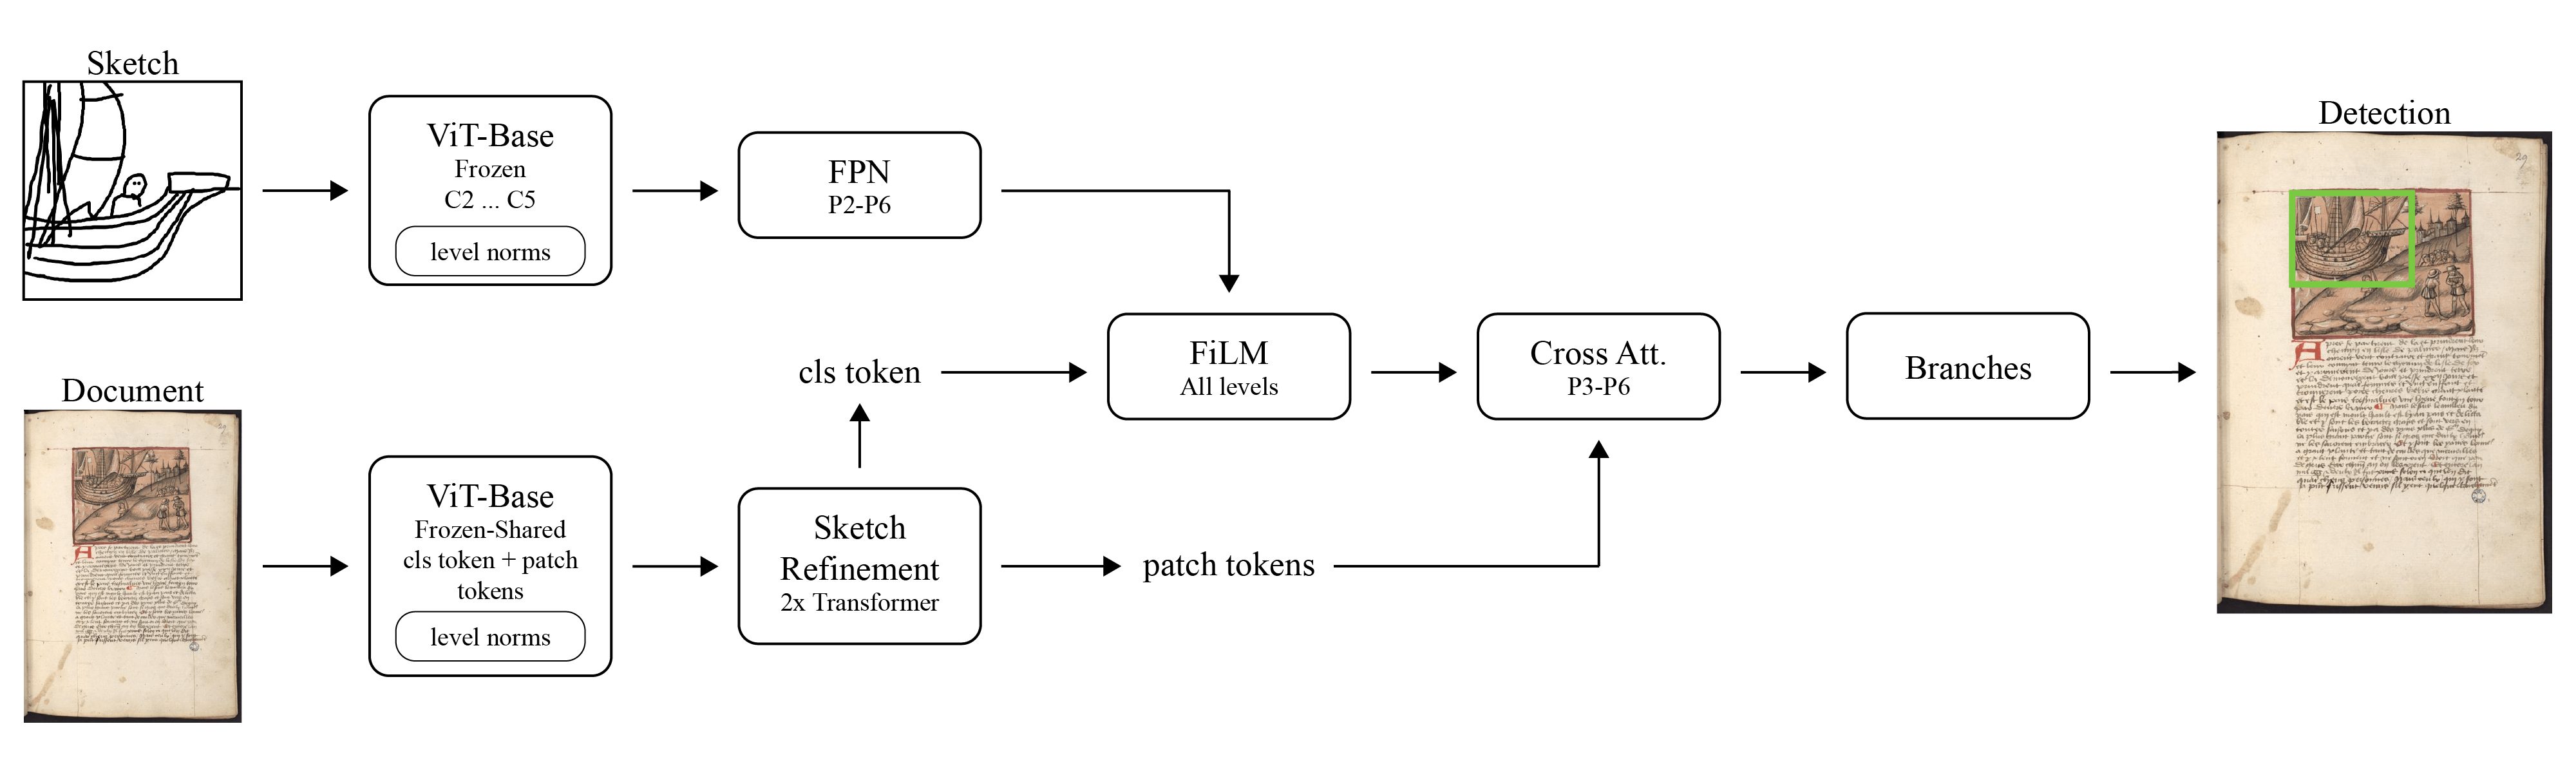
\includegraphics[width=0.9\textwidth]{images/architecture.png}
    \caption{General architecture of the proposed sketch-conditioned pattern spotting model. A frozen ViT backbone (iDoc or DINOv3) encodes the document page into multi-scale features through an FPN, while the same backbone encodes the sketch query into a global embedding and a set of local patch tokens, refined by a lightweight transformer encoder. Both sketch representations condition the FCOS detection head through FiLM and bidirectional co-attention, producing class, box, and centerness predictions at every pyramid level.} %% TODO: confirmar que la figura final realmente muestra esto
    \label{fig:architecture}
\end{figure}

\subsection{Architecture}

The backbone is a frozen Vision Transformer, either the iDoc encoder introduced in our previous work~\cite{saavedra2024idoc} or the more recent DINOv3~\cite{dinov3}, both supported transparently by detecting the structure of the checkpoint at loading time. Multi-scale features are obtained by extracting the token sequences at four intermediate blocks of the transformer and reshaping them into spatial maps $C_2$ through $C_5$, which are subsequently normalized by a small set of trainable LayerNorm layers to adapt the frozen representation to the detection task without modifying the backbone weights, and fed into a standard top-down Feature Pyramid Network~\cite{lin2017fpn} that produces the pyramid levels $P_2$ through $P_6$ used by the detection head.

The same frozen backbone is reused to encode the sketch query, producing a global class token and a set of patch tokens that are spatially pooled to a fixed grid to keep the cost of the subsequent attention operations manageable. Because the backbone was optimized for representing historical document patterns in general rather than for comparing a sketch against a specific image region, a lightweight, near-identity-initialized transformer encoder refines both the global and the local sketch representations before they are passed to the detection head, learning to emphasize the tokens that best discriminate the target shape from the background of the sketch.

The refined sketch representations condition the detection head through two complementary mechanisms. The global embedding modulates every pyramid level through a Feature-wise Linear Modulation (FiLM) layer~\cite{film2018}, providing a coarse, class-level prior at a negligible computational cost, while the local patch tokens interact with the document features through a bidirectional co-attention module applied from an intermediate pyramid level onward: the sketch representation first attends to the document features to adapt itself to the visual style of the current page, and the document features then attend to this contextualized sketch, sharpening the spatial regions that resemble the query.

On top of this conditioned representation, a standard FCOS head~\cite{fcos2019} predicts, at every location of every pyramid level, a classification score, a bounding box expressed as the distance to the four sides of the object, and a centerness score that down-weights predictions far from the object center; the final detection score is the product of the sigmoid of the classification and centerness predictions. The model is trained end to end with a combination of focal loss for classification, generalized IoU loss for box regression, and binary cross-entropy for centerness, complemented by a supervised contrastive loss~\cite{khosla2020supcon} over the global sketch embeddings of the batch, which compacts the representation of sketches belonging to the same class and is particularly useful for the long tail of categories with very few annotated examples.

Training proceeds in two stages: the new sketch-conditioning modules are first optimized in isolation while the rest of the network remains frozen, and the whole detector is then fine-tuned jointly with a lower learning rate for the previously converged components, which we found to stabilize the introduction of the conditioning mechanisms without disrupting the pattern-spotting capability inherited from~\cite{saavedra2024idoc}. At inference time, an adaptive score threshold raises the operating point in densely decorated pages to suppress the long tail of weak activations, and a context-aware non-maximum suppression step further removes clusters of similarly-scored detections that are characteristic of repetitive textures rather than genuine objects; when more than one sketch example of the same class is available, their embeddings can also be averaged into a single prototype to reduce the influence of idiosyncratic strokes.

\subsection{Dataset}
 
%% TODO: siguen faltando dos datos que el reporte de auditoria no cubre: (1) el origen/fuente del corpus -- claramente NO es DocExplore tal cual (que tiene 1500 paginas y 35 clases), asi que aclarar si es un subconjunto/extension de DocExplore, de HORAE, o un corpus nuevo curado para este trabajo; (2) el protocolo de recoleccion de los sketches de query (cuantos por clase, dibujados por quien, en que herramienta/soporte).
We evaluate our proposal on a dataset of 544 historical document pages [COMPLETAR: fuente del corpus], annotated with 1{,}349 bounding boxes spanning 22 classes of recurring graphical patterns, with an average of 2.48 annotated instances per page and no invalid (zero-area) boxes found during the audit. Table~\ref{tab:class_distribution} summarizes the class distribution. The class distribution is severely long-tailed (Gini index of 0.537): the most frequent class, \textit{marqeur}, alone accounts for 32.2\% of all instances (434 occurrences), while 17 of the 22 classes (77\%) contain fewer than 50 labeled examples, with the two rarest classes counting only 7 instances each; this imbalance directly motivates the supervised contrastive loss and the class-aware copy-paste augmentation described above.
 
\begin{table}[htb]
\centering
\caption{Class distribution and median instance area in the annotated dataset (544 pages, 1{,}349 bounding boxes, 22 classes).}
\label{tab:class_distribution}
\begin{tabular}{lrrr}
\toprule
Class & $N$ & \% & Median area (px$^2$) \\
\midrule
marqeur      & 434 & 32.17 & 741.0 \\
S            & 138 & 10.23 & 1{,}272.5 \\
losange      & 117 & 8.67  & 3{,}306.0 \\
double\_sep  & 98  & 7.26  & 1{,}572.5 \\
croix        & 91  & 6.75  & 1{,}248.0 \\
petit\_A     & 49  & 3.63  & 1{,}512.0 \\
encadrement  & 45  & 3.34  & 6{,}750.0 \\
obj\_1       & 39  & 2.89  & 11{,}016.0 \\
pdp          & 35  & 2.59  & 1{,}200.0 \\
status       & 34  & 2.52  & 16{,}371.0 \\
obj\_61      & 34  & 2.52  & 9{,}743.5 \\
T            & 32  & 2.37  & 1{,}500.0 \\
grand\_A     & 31  & 2.30  & 3{,}700.0 \\
obj\_2       & 31  & 2.30  & 358{,}515.0 \\
BP           & 28  & 2.08  & 19{,}773.0 \\
obj\_40      & 25  & 1.85  & 10{,}925.0 \\
obj\_34      & 24  & 1.78  & 31{,}010.5 \\
triple\_sep  & 20  & 1.48  & 3{,}960.0 \\
obj\_37      & 16  & 1.19  & 10{,}536.0 \\
obj\_39      & 14  & 1.04  & 7{,}198.0 \\
obj\_42      & 7   & 0.52  & 73{,}502.0 \\
obj\_31      & 7   & 0.52  & 30{,}504.0 \\
\bottomrule
\end{tabular}
\end{table}
 
Beyond class frequency, the annotated patterns also exhibit substantial geometric variability, as illustrated in Fig.~\ref{fig:variability}: instance width and height range from 13 to over 3{,}000~px, with area spanning more than four orders of magnitude (from 234~px$^2$ to $3.1\times10^{6}$~px$^2$); the median instance is small and moderately horizontal (50$\times$28~px, aspect ratio 1.73). Following the standard COCO size convention, 30.7\% of the instances are small (area below $32^2$~px), 54.6\% are medium ($32^2 \leq$ area $< 96^2$~px), and 14.7\% are large (area $\geq 96^2$~px); aspect ratios are skewed toward horizontal shapes, with 72.9\% of instances above $\mathrm{AR}=1.2$ (35.0\% of them extremely so, $\mathrm{AR}>2$), against 16.5\% near-square instances and only 10.6\% vertical ones.
 
This variability is intrinsic to the semantics of the illustrations themselves, since the size and aspect ratio of a graphical pattern depend on the type of object it represents, its relative importance within the composition, and the amount of detail the scribe or illuminator devoted to it.

\begin{figure}[htb]
    \centering
    \begin{subfigure}[b]{0.45\textwidth}
        \centering
        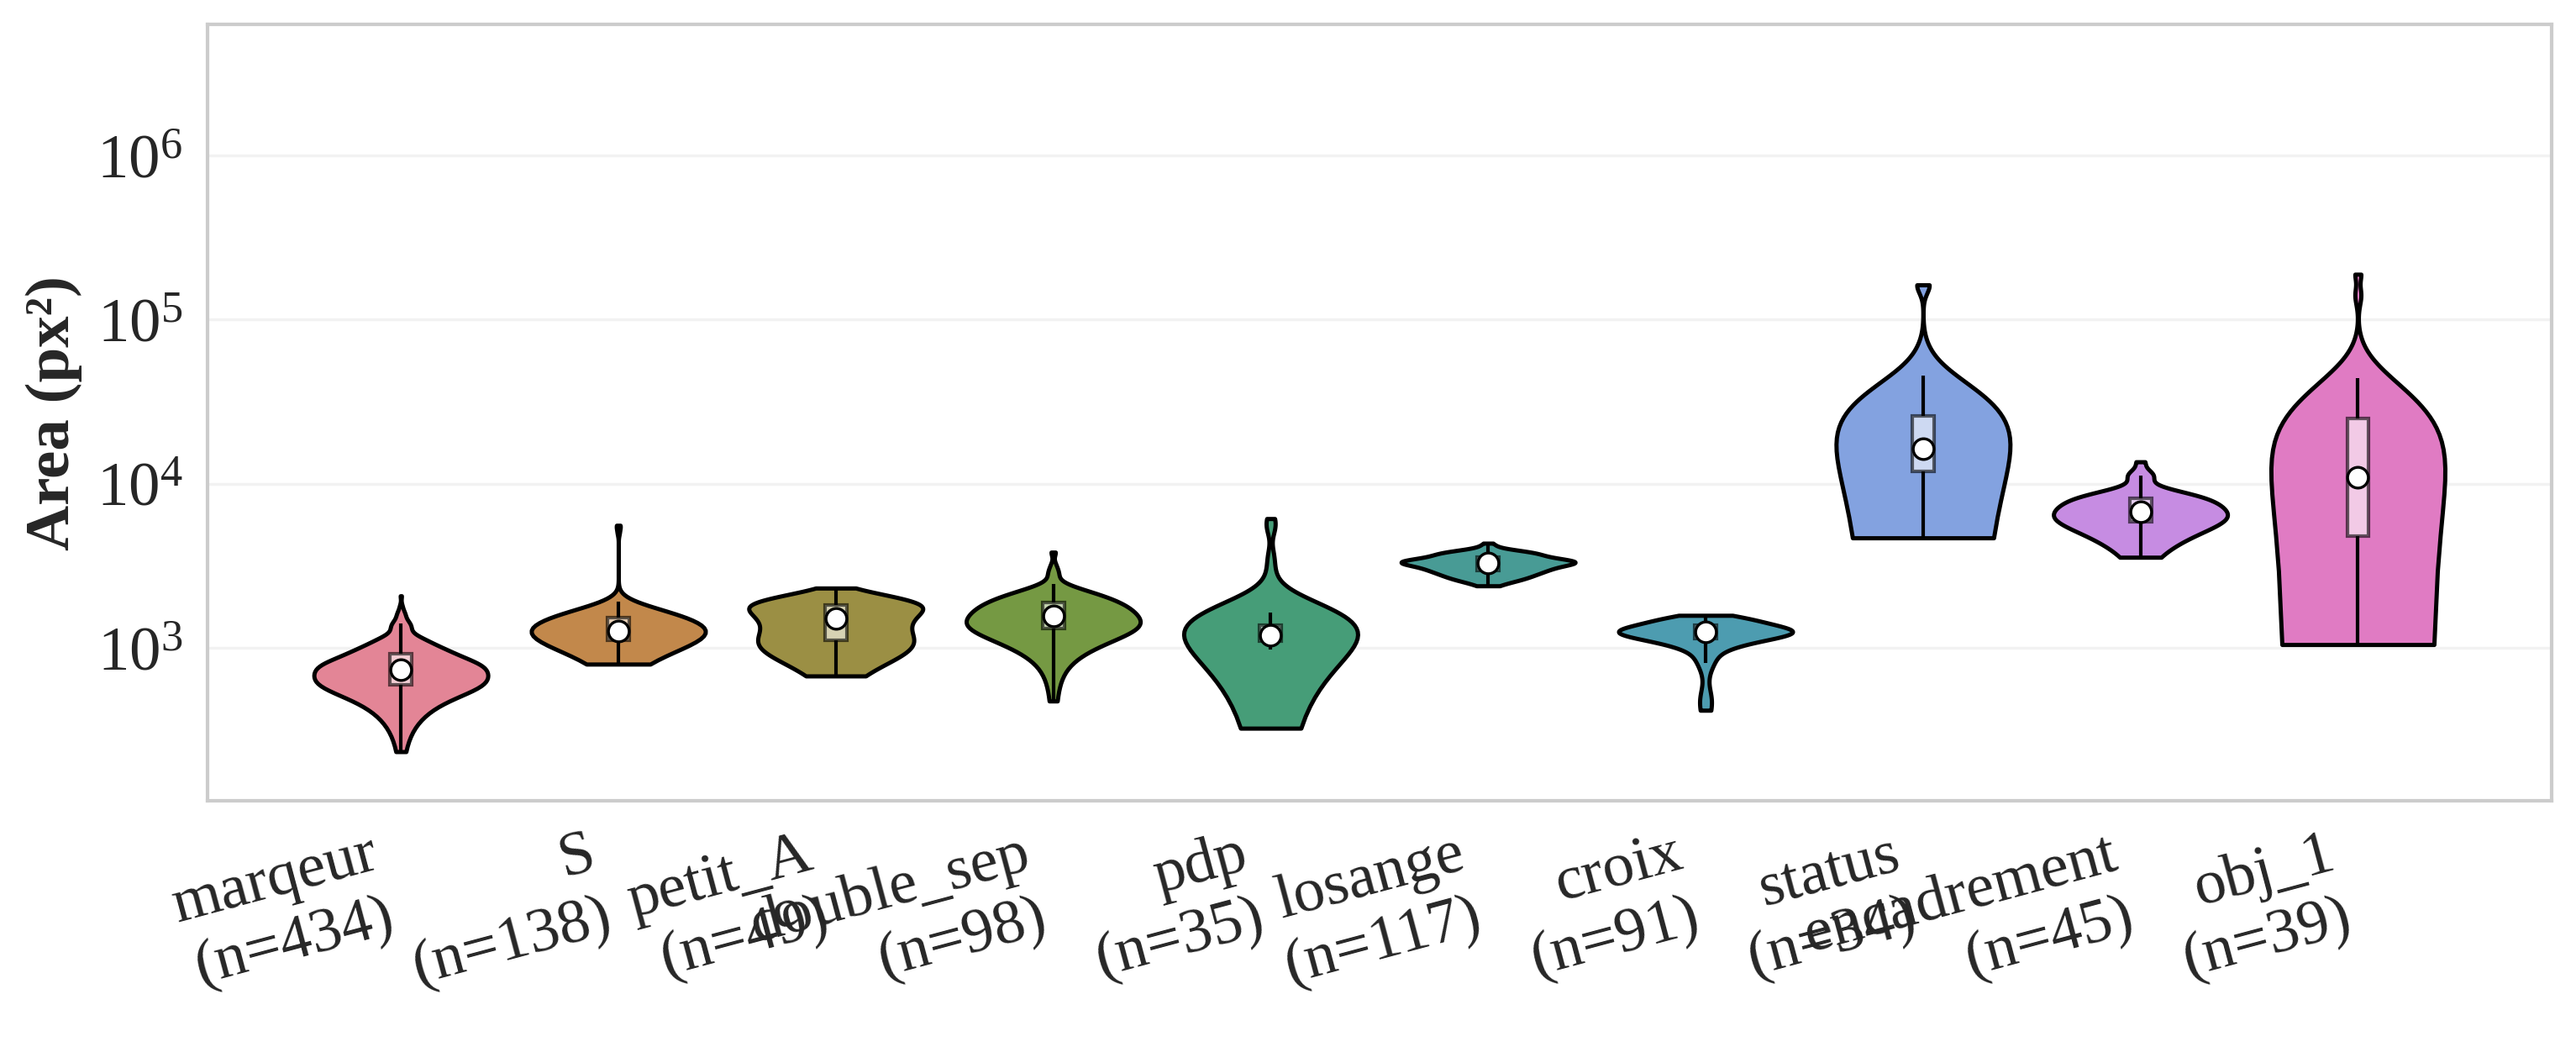
\includegraphics[width=\textwidth]{images/fig1_bbox_area_dist.png}
        \caption*{(a)}
    \end{subfigure}
    \hspace{10pt}
    \begin{subfigure}[b]{0.45\textwidth}
        \centering
        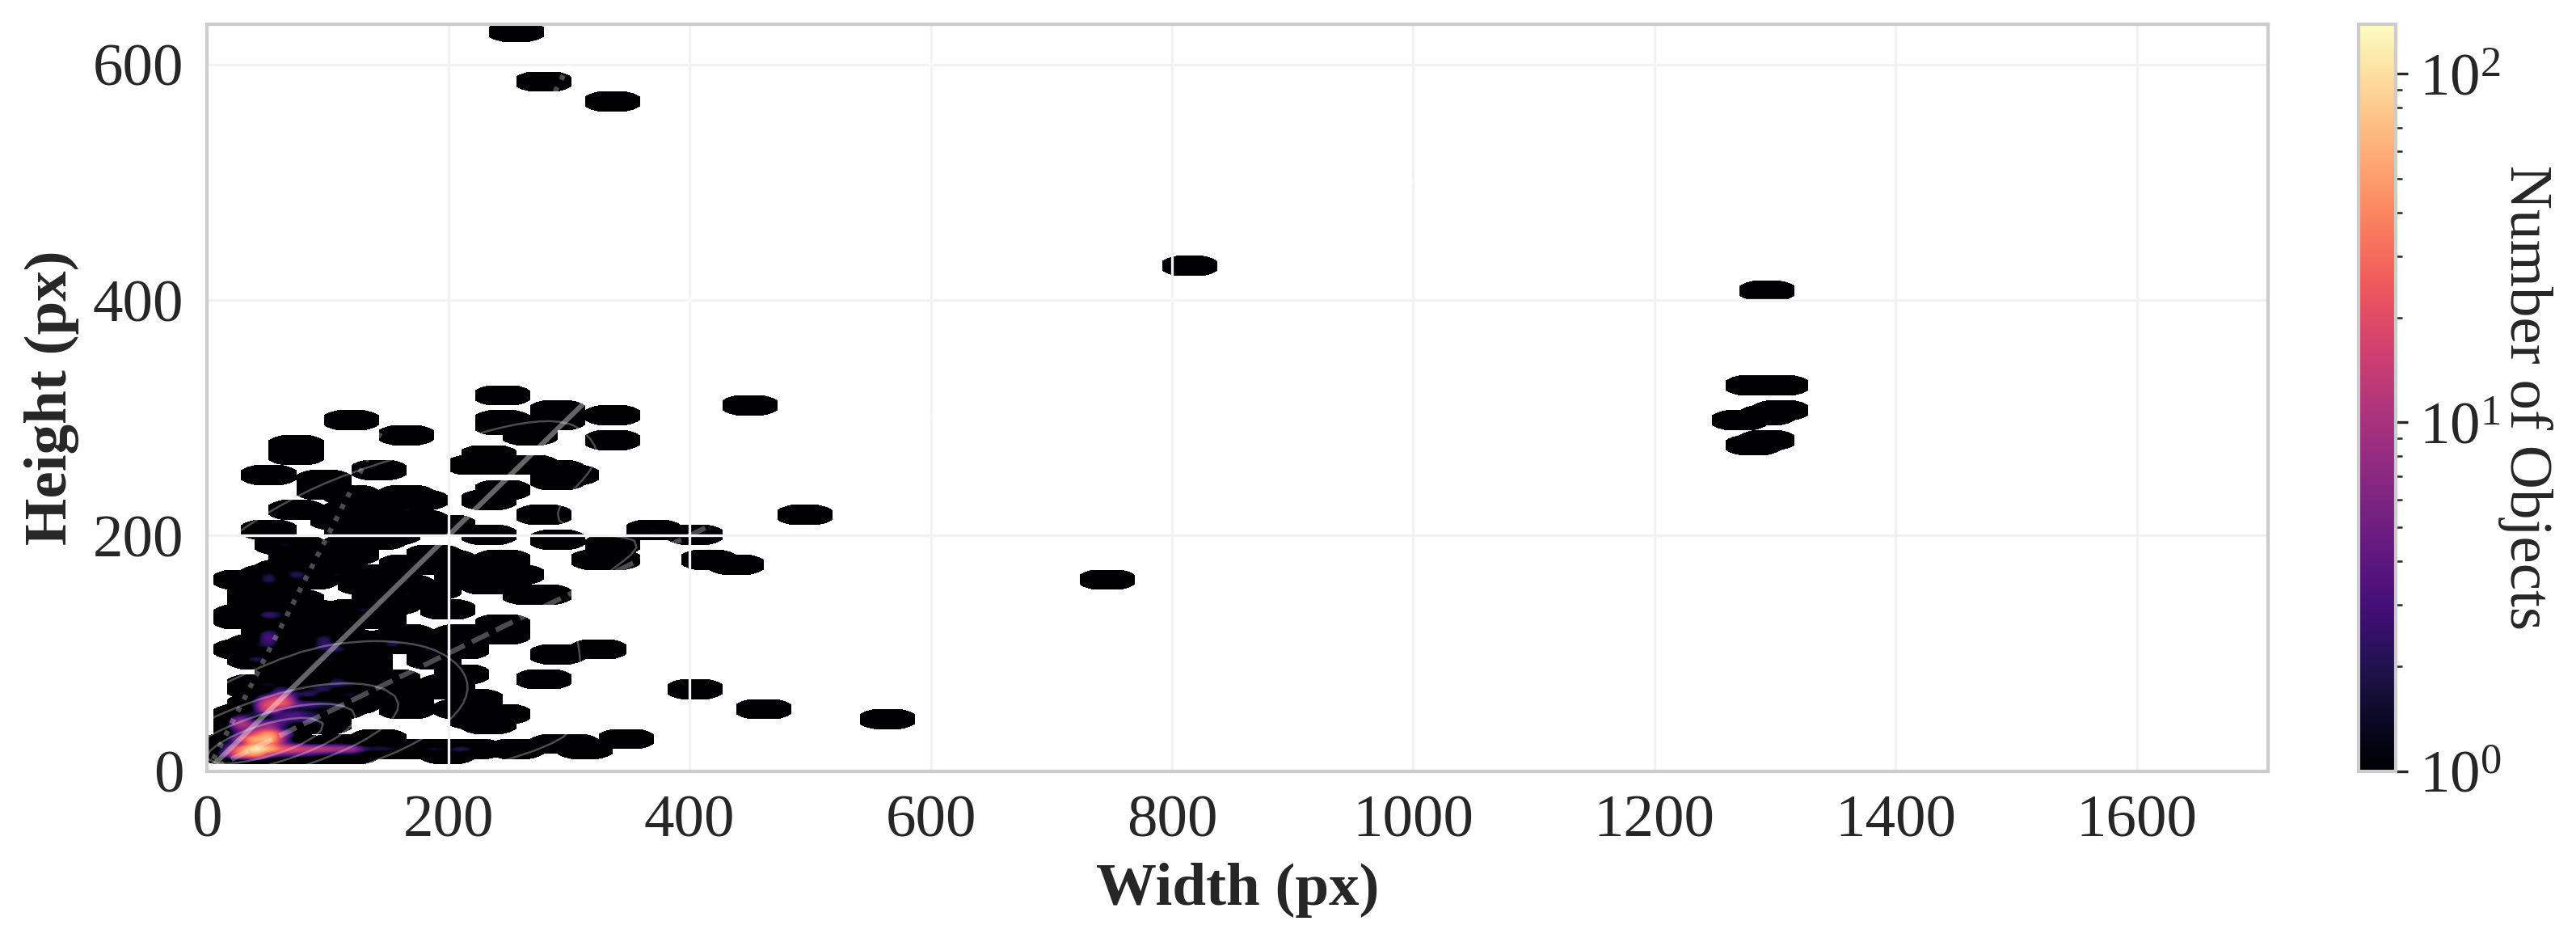
\includegraphics[width=\textwidth]{images/fig2_bbox_dimensions_heatmap.png}
        \caption*{(b)}
    \end{subfigure}
    \caption{\textcolor{red}{REDACTAR}}
    \label{fig:variability}
\end{figure}
 
Beyond this geometric variability, the sketch-conditioned setting introduces three additional sources of difficulty that directly motivated the design choices described above: most classes have very few annotated instances, which limits the supervision available for learning a discriminative sketch representation; the same symbol can vary considerably in appearance across pages and scribes, so a single sketch may not be representative of every occurrence; and densely decorated pages contain repetitive textures and ornaments that are easily confused with the target pattern, leading to a large number of false positives if left unaddressed.

% ─────────────────────────────────────────────────────────────────────────────
%  SECTION: Experimental Results
%  Paste this block after \subsection{Dataset} in main.tex
% ─────────────────────────────────────────────────────────────────────────────

\section{Experimental Results}

Table~\ref{tab:global_results} summarizes the overall detection performance of both
backbone variants on the validation split (55 pages, 111 ground-truth boxes) at
IoU$\,{=}\,0.50$ and a score threshold of $0.25$.
DINOv3-FCOS outperforms iDoc-FCOS across every reported metric, achieving a
mean Average Precision of $0.701$ against $0.582$ for iDoc ($+12$ points), while
simultaneously reducing the false-positive rate from $26.5\%$ to $17.9\%$ and
raising recall from $74.8\%$ to $86.5\%$.
This result is noteworthy because iDoc was explicitly adapted to the historical
document domain via LoRA fine-tuning on the HORAE corpus~\cite{saavedra2024idoc},
whereas DINOv3 is a general-purpose encoder.
The gap suggests that, when the backbone is used as a frozen feature extractor
for a trainable detection head rather than as a similarity-search encoder, the
richer, more diverse representations learned by DINOv3 transfer more effectively
to the sketch-conditioned FCOS head than the more narrowly specialized
representations of iDoc.

\begin{table}[htb]
\centering
\caption{Global detection metrics for both backbone variants on the validation
split (55 pages, 111 ground-truth boxes, IoU\,=\,0.50, score\,thr.\,=\,0.25).
$\Delta$ denotes the absolute gain of DINOv3-FCOS over iDoc-FCOS.}
\label{tab:global_results}
\begin{tabular}{lrrr}
\toprule
Metric & iDoc-FCOS & DINOv3-FCOS & $\Delta$ \\
\midrule
mAP @ IoU=0.50 & 0.582 & \textbf{0.701} & $+0.119$ \\
Precision       & 0.735 & \textbf{0.821} & $+0.086$ \\
Recall          & 0.748 & \textbf{0.865} & $+0.117$ \\
F1              & 0.741 & \textbf{0.842} & $+0.101$ \\
\midrule
Total TP        &  83   & \textbf{96}    & $+13$    \\
Total FP        &  30   & \textbf{21}    & $-9$     \\
Total FN        &  28   & \textbf{15}    & $-13$    \\
FP rate         & 26.5\% & \textbf{17.9\%} & $-8.6$\,pp \\
\bottomrule
\end{tabular}
\end{table}

\subsection{Per-Class Analysis}

Table~\ref{tab:per_class_results} reports Average Precision (AP) per class for
the 15 classes that have at least one ground-truth instance in the validation
split; the remaining 7 classes are absent from the split and cannot be evaluated.

\begin{table}[htb]
\centering
\caption{Per-class Average Precision (AP) at IoU\,=\,0.50.
GT denotes the number of ground-truth boxes in the validation split.
Classes marked with ($\bullet$) have no ground-truth instances in the split
and are excluded.
Best result per class in \textbf{bold}.}
\label{tab:per_class_results}
\begin{tabular}{lrrr}
\toprule
Class & GT & iDoc-FCOS & DINOv3-FCOS \\
\midrule
marqeur      & 60 & 0.858          & \textbf{0.860} \\
S            &  6 & 0.732          & \textbf{1.000} \\
double\_sep  &  8 & 0.899          & \textbf{1.000} \\
losange      &  4 & \textbf{1.000} & \textbf{1.000} \\
grand\_A     &  6 & \textbf{1.000} & \textbf{1.000} \\
petit\_A     &  4 & 0.883          & \textbf{1.000} \\
obj\_34      &  3 & \textbf{1.000} & 0.909          \\
T            &  3 & \textbf{0.727} & 0.636          \\
BP           &  1 & \textbf{0.333} & 0.250          \\
status       &  4 & 0.245          & \textbf{0.636} \\
obj\_2       &  3 & 0.500          & \textbf{0.636} \\
obj\_42      &  2 & 0.182          & \textbf{0.628} \\
obj\_39      &  2 & 0.000          & \textbf{0.545} \\
obj\_61      &  4 & 0.273          & \textbf{0.409} \\
obj\_37      &  1 & 0.100          & 0.000          \\
\midrule
\multicolumn{2}{l}{Classes with AP$\,{\geq}\,0.50$} & 8 / 22 & \textbf{12 / 22} \\
\bottomrule
\end{tabular}
\end{table}

The class-level results reveal a more nuanced picture than the aggregate metrics
alone suggest.
For high-frequency or geometrically simple classes \textit{losange},
\textit{grand\_A}, \textit{obj\_34}, and \textit{T} iDoc-FCOS is competitive
with or superior to DINOv3-FCOS, indicating that the domain-adapted
representation is advantageous when ample training signal is available and
the target shape is relatively unambiguous.
Conversely, DINOv3-FCOS achieves substantially higher AP on rare and visually
complex classes, including \textit{status} ($+0.391$), \textit{obj\_42}
($+0.446$), \textit{obj\_39} ($+0.545$), and \textit{S} ($+0.268$), suggesting
that the broader feature vocabulary of the general-purpose encoder generalizes
better to the long tail of the class distribution.
This observation is consistent with the hypothesis that domain adaptation narrows
the representation toward patterns that are statistically dominant in the
training corpus, at the cost of coverage over rare or atypical categories.

Regarding false positives, iDoc-FCOS generates $43\%$ more false
detections than DINOv3-FCOS (30 vs.\ 21).
The most pronounced cases are \textit{petit\_A}, where iDoc produces 6
false positives against 4 true positives (precision 0.40), and \textit{BP},
where it produces 4 false positives with a single true positive.
DINOv3-FCOS, despite producing false positives of its own on these classes,
ranks its predictions more reliably, as reflected in the higher AP scores.

Finally, seven classes \textit{croix}, \textit{encadrement}, \textit{obj\_1},
\textit{obj\_31}, \textit{obj\_40}, \textit{pdp}, and \textit{triple\_sep} are
entirely absent from the validation split, preventing their evaluation.
This is a direct consequence of the severe class imbalance in the dataset
(Gini index 0.537; see Table~\ref{tab:class_distribution}) and motivates the use
of stratified splitting in future work to ensure every class is represented in
all partitions.


\section{Conclusions}
 
We have presented a sketch-conditioned, one-stage detector for pattern spotting
in historical documents that bridges, for the first time at scale, the
paradigms of sketch-based image retrieval and graphical pattern localization.
By conditioning a standard FCOS detection head on a hand-drawn sketch through a
combination of FiLM modulation and bidirectional co-attention, the proposed
system can localize recurring graphical patterns in medieval manuscript pages
without requiring any example image of the target, relying solely on a query
drawn by the user.
 
The comparative evaluation of two frozen ViT backbones yields a clear and
somewhat surprising finding: DINOv3-FCOS achieves a mAP of $0.701$, outperforming
iDoc-FCOS ($0.582$) by $+12$ points despite the fact that iDoc was explicitly
adapted to the historical document domain.
The advantage of DINOv3 is most pronounced for rare and visually complex classes
(\textit{status}, \textit{obj\_42}, \textit{obj\_39}), where its broader
feature vocabulary appears to generalize better to the long tail of the class
distribution.
iDoc-FCOS, by contrast, remains competitive on high-frequency and geometrically
simple classes (\textit{losange}, \textit{grand\_A}, \textit{obj\_34}),
suggesting that domain adaptation is beneficial when sufficient training signal
is available but does not compensate for the reduced representational diversity
in low-resource regimes.
This result implies that, when the backbone is used as a frozen feature
extractor for a trainable detection head rather than as a direct
similarity-search encoder, diversity of pre-training data matters more than
domain specificity.
 
Several directions for future work remain open.
First, the severe class imbalance in the dataset (Gini index $0.537$) prevents
the evaluation of seven classes in the current validation split; stratified
cross-validation would provide a more comprehensive and reliable estimate of
per-class performance.
Second, the contrastive loss and the copy-paste augmentation, which were
specifically motivated by the long-tail distribution, warrant a dedicated
ablation study to quantify their individual contributions.
Third, the detection head currently conditions on a single sketch per query;
extending the prototype averaging strategy to multiple sketches per class, and
studying how the number and diversity of sketches affect localization accuracy,
would make the system more robust to idiosyncratic drawing styles.
Finally, end-to-end fine-tuning of the backbone with a low learning rate,
or lightweight adaptation via LoRA applied directly within the detection
pipeline, may further close the gap between the two encoder variants and
improve performance on the most challenging classes.

\bibliographystyle{unsrt}
\bibliography{references}


\end{document}